\chapter{Měření}
\label{chap:benchmark}
Náš projekt se skládá ze dvou částí a to hry a poté měření, které využívá vytvořenou hru pro měření výkonu jednotlivých ECS knihoven. Analýzu tohoto měření jsme provedli v sekci~\ref{benchmark-analysis} a jeho implementaci jsme popsali v sekci~\ref{benchmark-implementation}. V této kapitole si nejprve ukážeme jak lze měření spustit, následně si stanovíme hypotézu, poté si přiblížíme ECS knihovny, které budeme měřit a na závěr si prezentujeme výsledky tohoto měření.

\section{Spouštění měření}
Mezi přílohami projektu~\ref{chap:attachments} lze najít adresář \texttt{src} obsahující zdrojové soubory a sestavený projekt měření. Pomocí aplikace \texttt{src\textbackslash WorldSimulator.BenchMarks\textbackslash bin\textbackslash Release\textbackslash net7.0\textbackslash WorldSimulator.Benchmarks.exe} lze spustit měření. Pro úpravu parametrů měření je potřeba upravit a znovu sestavit zdrojový kód. Fieldy relevantní k měření je možné nalézt v tabulce~\ref{tab:benchmark-relevant-fields}. Pro každý field je v této tabulce zobrazen jeho název a poté jeho popis. První čtyři z těchto fieldů se nacházejí ve třídě \texttt{WorldSimulator.BenchMarks.ECSBenchmarks}. Poslední z nich se nachází ve třídě \texttt{WorldSimulator.Level.World}.

\begin{table}[!htb]
    \centering\footnotesize\sf
    \begin{tabular}{c c}
        \toprule
        název fieldu & popis fieldu \\
        \midrule

        \texttt{seed} & Seed pro generování náhodných čísel. \\

        \texttt{deltaTime} & Odsimulovaný čas mezi dvěma iteracemi \textit{game loop}. \\

        \texttt{setupIterationCount} & Počet iterací \textit{game loop} během warmup fáze. \\

        \texttt{benchmarkIterationCount} & Počet iterací \textit{game loop} během měření. \\

        \texttt{Size} & Výška a šířka herního světa. \\
        \bottomrule
    \end{tabular}
    \caption{Seznam fieldů relevantních k měření.}
    \label{tab:benchmark-relevant-fields}
\end{table}

\section{Hypotéza}
\label{chap:hypothesis}
V této sekci si stanovíme hypotézu našeho měření. V našem měření měříme jak dlouho trvá odsimulovat určitý počet iterací naší hry s jednotlivými ECS knihovnami. Ty se dají rozdělit na kategorie podle určitých vlastností. V této kapitole stanovíme jak si myslíme, že se jednotlivé kategorie umístí.

% Do teď jsme se věnovali samotné hře, kterou v následujících kapitolách budeme chtít použít pro porovnání výkonu ECS knihoven. Ale ještě předtím, konkrétně v této kapitole, si rozebereme předpokládané výsledky tohoto porovnání.

\subsection{Cache}
Využití cache je klíčový faktor pro výkon ECS knihovny, proto si nyní připomene co to vlastně je a jak funguje.

Program si svoje data uchovává v paměti RAM. Ovšem přístup do této paměti je z hlediska času drahý. Pro představu u moderních pamětí takovíto přístup může trvat vyšší desítky nanosekund. Z tohoto důvodu se využívají menší paměti, takzvané cache, které disponují mnohem vyšší rychlostí ale mnohem menší velikostí. Pro představu moderní procesory používají cache, u kterých přístup může trvat menší desetiny nanosekund.

Při přístupu k datům se procesor nejprve podívá zda nemá data již v této cache. Pokud ano, jedná se o takzvaný \textit{cache hit} a data si z ní načte. Pokud ne, jedná se o takzvaný \textit{cache miss} a je nutné data načíst z hlavní paměti. 

Již víme, že \textit{cache miss} jsou drahé, proto je potřeba pro vysoký výkon je minimalizovat. Ale jak přesně procesor rozhoduje o tom, jaká data budou v cache a jaká ne. Využívá se takzvané \textit{časové} a \textit{prostorové lokality}. \textit{Časová lokalita} spočívá v tom, že pokud jsme přistoupili k nějakým datům, je velká šance, že k nim brzo budeme chtít přistoupit znovu. Nadruhou stranu \textit{prostorová lokalita} spočívá v tom, že pokud jsme přistoupili k nějakým datům, je velká šance, že budeme chtít přistoupit také k datům, které se nacházejí blízko nich.

Jedna z možností, jak minimalizovat počet \textit{cache miss}, je využít sekvenčního přístupu. Pokud budeme přistupovat k datům, které jsou v paměti hned za sebou, tak díky \textit{prostorové lokalitě} bude počet \textit{cache miss} velmi malí.

Je nutné upozornit, že výše popsaný model cache je úmyslně zjednodušen. Velice detailní popis cache lze nalézt v \textit{Cache Memories}~\cite{10.1145/356887.356892} od \textit{Alana Jaye Smitha}. Stručnější popis a také informace o tom jak lze cache využít lze nalézt v již zmiňované knize \textit{Game Programming Patterns}~\cite{nystrom2014game}, konkrétně v kapitole \textit{Data Locality}. 

\subsection{Arch type}
Některé ECS knihovny pro lepší výkon používají \textit{arch type}. Jedná se o datovou strukturu pro ukládání komponent. Knihovny, které používají tuto datovou strukturu mají většinou velký výkon, proto před stanovením hypotézy si použití \textit{arch type} lehce přiblížíme.

Jak již bylo zmíněno, \textit{arch type} je datová struktura. Tato datová struktura představuje typ entity. Tento typ je jednoznačně určen typy všech komponent dané entity. Je možné si jej představit jako tabulku, kde jednotlivé sloupečky odpovídají komponentám a v každém řádku se nacházejí instance komponent pro danou entitu. Například můžeme mít \textit{arch type} vyobrazený v tabulce~\ref{tab:arch-type}. Tento \textit{arch type} je jednoznačně určen typy komponent \texttt{Position} (představující pozici entity), \texttt{Health} (představující počet životů entity) a \texttt{Damage} (představující poškození, které entita může udělit jiné entitě).

\begin{table}[!htb]
    \centering\footnotesize\sf
    \begin{tabular}{c c c c}
        \toprule
        entita & \texttt{Position} & \texttt{Health} & \texttt{Damage} \\
        \midrule
        hráč & $(0,0)$ & 10 & 3 \\
        nepřítel & (5,4) & 6 & 1 \\
        npc & (-4,8) & 16 & 9\\
        \bottomrule
    \end{tabular}
    \caption{Tabulka vyobrazující \textit{arch type}, který je jednoznačně určen komponentami \texttt{Position}, \texttt{Health} a \texttt{Damage}. Tento \textit{arch type} obsahuje tři entity, konkrétně hráče, nepřítele a npc.}
    \label{tab:arch-type}
\end{table}

Jednotlivé \textit{arch type} jsou uloženy ve \textit{world}. Každý \textit{arch type} má v sobě několik polí, konkrétně jedno pole pro každý typ komponenty. V každém poli jsou poté uloženy instance příslušných komponent. V případě \textit{arch type} z tabulky~\ref{tab:arch-type} by tento \textit{arch type} obsahoval jedno pole pro \texttt{Position} komponenty, jedno pole pro \texttt{Health} komponenty a jedno pole pro \texttt{Damage} komponenty.

Pokud bychom chtěli iterovat přes všechny entity s danými komponentami, stačilo by nám projít příslušná pole všech \textit{arch type} s těmito komponentami. Tato iterace by byla, díky sekvenčnímu přístupu zmíněnému v minulé sekci, velice rychlá. Ke \textit{cache miss} by docházelo pouze při přechodu na další \textit{arch type}.

Nevýhodou knihoven založených na \textit{arch type} bývá pomalé přidávání a odebírání komponent. Pokud je entitě přidána nebo odebrána komponenta, dojde ke změně jejího \textit{arch type}. Při této změně se vezmou instance všech komponent dané entity a přesunou se do nového \textit{arch type}.

Pro více informací o \textit{arch type} a o tom jak je ECS knihovny využívají je možné nahlédnout do série článků \textit{ECS back and forth}~\cite{Caini_2019} od Michela Cainiho.

\subsection{Stanovení hypotézy}
\label{hypothesis}
Nyní stanovíme hypotézu. Jednotlivé ECS knihovny lze rozdělit do kategorií na základě jistých vlastností. My tyto kategorie popíšeme a stanovíme jaké bude jejich pořadí při výkonnostním porovnání.

Nejrychleji vyjdou ECS knihovny, které vyžadují aby byli komponenty reprezentovany jako struktury a zároveň používají \textit{arch type}. Jak již bylo zmíněno, díky sekvenčnímu přístupu, který \textit{arch type} využívá, dojde k minimalizaci počtu \textit{cache miss}. To má za následek vysoký výkon. Z toho důvodu tyto knihovny vyjdou nejlépe. Označme tuto kategorii jako kategorii 1.

Některé ECS knihovny vyžadují, aby jednotlivé komponenty, byli reprezentovány jako třídy. Tyto knihovny vyjdou nejhůře. V případě, že komponenta je třída, znamená to, že její proměnné musejí být pointery. Z toho důvodu iterace přes komponenty v těchto knihovnách vede ve velmi velký počet \textit{cache miss}, kvůli kterému se tyto knihovny umístí nejhůře. Označme tuto kategorii jako kategorii~3.

Zbývají knihovny, které používají \textit{arch type} a zároveň vyžadují aby komponenty byli reprezentovány jako třídy. Tyto knihovny se umístí hůře než knihovny z kategorie 1, ale lépe než knihovny z kategorie 3. Označme tuto kategorii jako kategorii 2.

\section{Měřené knihovny}
V této sekci se budeme zabývat ECS knihovnami, které budeme měřit. První si uvedeme odkud měřené ECS knihovny bereme a poté si jednotlivé ECS knihovny krátce představíme.

V sekci~\ref{sec:ecs-libs} jsme zmínili, že existuje repositář \textit{EcsCsharpBenchmark}~\cite{EcsCsharpBenchmark} na platformě GitHub obsahující výkonnostní porovnání ECS knihoven pro C\#. Tento repositář byl inspirací této práce, která také porovnává jednotlivé ECS knihovny, ale na místo jednoduchých testů je porovnává na hře. V našem měření budeme měřit knihovny, které byli porovnávány ve zmiňovaném repositáři \textit{EcsCsharpBenchmark}~\cite{EcsCsharpBenchmark}.

Od zahájené této práce byl repositář \textit{EcsCsharpBenchmark}~\cite{EcsCsharpBenchmark} několikrát upraven. Během úprav byli přidávány a odebírány některé ECS knihovny z porovnání. V této práci se zaměříme na knihovny, které byli v repositáři \textit{EcsCsharpBenchmark}~\cite{EcsCsharpBenchmark} porovnávány během commitu \textit{db67d1d}~\cite{EcsCsharpBenchmarkCommit}.

Nyní si představíme jednotlivé ECS knihovny, které budeme měřit. U každého si uvedeme přeložený popisek, který je možné nalézt v repositáři dané knihovny. Tyto popisky jsou doslovně převzaté a autor práce neručí za korektnost informací, které jsou jejich obsahem.

\begin{enumerate}
    \item \textbf{Arch~\cite{Arch}:} Vysoko-výkonnostní ECS knihovna založená na Archtype a Chunks určená pro herní vývoj a data-oriented programování.
    \item \textbf{DefaultEcs~\cite{DefaultEcs}:} ECS framework, který si klade za cíl být přístupný s minimálními omezeními, zatímco zachovává co největší výkon pro vývoj her.
    \item \textbf{Entitas~\cite{Entitas}:} Nejpopulárnější open-source ECS framework pro C\# a Unity.
    \item \textbf{HypEcs~\cite{HypEcs}:} Lightweight a snadno použitelná ECS knihovna s efektivní sadou funkcionalit pro tvorbu her.
    \item \textbf{LeoECS~\cite{LeoECS}:} Lightweight ECS framework pro C\#. Mezi hlavní cíle tohoto frameworku patří výkon, nulová nebo minimální alokace, minimalizace využití paměti a absence závislostí na jakémkoliv herním enginu. (Přeloženo pomocí ChatGPT.)
    \item \textbf{LeoEcsLite~\cite{LeoEcsLite}:} Lightweight ECS framework pro C\#. Mezi hlavní cíle tohoto frameworku patří výkon, nulová nebo minimální alokace, minimalizace využití paměti a absence závislostí na jakémkoliv herním enginu. (Přeloženo pomocí ChatGPT.)
    \item \textbf{MonoGameExtended.Entities~\cite{MonoGameExtended}:} Moderní vysoce výkonnostní ECS framework založený na Artemis.
    \item \textbf{RelEcs~\cite{RelEcs}:} Lightweight a snadno použitelná ECS knihovna s efektivní sadou funkcionalit pro tvorbu her.
    \item \textbf{Svelto.ECS~\cite{SveltoECS}:} Reálný ECS framework pro C\#. Umožňuje psát zapouzdřený, oddělený, udržovatelný, vysoce efektivní, datově orientovaný, cache-přátelský kód bez bolesti.
\end{enumerate}

V minulé sekci jsme si definovali kategorie do kterých jednotlivé ECS knihovny spadají. Do kategorie 1 patří \textit{Arch}, \textit{HypEcs} a \textit{Svelto.ECS}. Do této kategorie také zařadíme \textit{DefaultEcs}, \textit{LeoECS} a \textit{LeoEcsLite}, které sice \textit{arch type} nepoužívají, ale používají datovou strukturu, která také využívá sekvenčního přístupu pro minimalizaci počtu \textit{cache miss}. V kategorii 2 je pouze \textit{RelEcs}. Do kategorie 3 spadají \textit{MonoGameExtended.Entities} a \textit{Entitas}.

\section{Výsledky}
\label{sec:benchmark-results}
Analýzu měření jsme provedli v sekci~\ref{benchmark-analysis}. Poté v sekci~\ref{benchmark-implementation} jsme si rozebrali implementaci měření. V této sekci se budeme věnovat výsledkům tohoto měření.

Předtím něž si prezentujeme výsledky měření, tak si shrňme jak jej provádíme. Prvně si vytvoříme novou instanci hry (instanci třídy \texttt{Game}) s danou ECS knihovnou (s danou instancí třídy dědicí od \texttt{ECSFactory}). Poté odsimulujeme přípravný počet iterací (provedeme \texttt{setupIterationCount} iterací \textit{game loop} naší hry). Následně odsimulujeme měřený počet iterací (\texttt{benchmarkIterationCount}) a přitom budeme měřit čas. To několikrát zopakujeme (přesněji námi zvolený framework to za nás několikrát zopakuje) a získáme průměrný čas jak rychle hra zvládne odsimulovat měřený počet iterací (\texttt{benchmarkIterationCount}). Test provádíme pro každou měřenou ECS knihovnu (ty jsme si rozebrali v minulé sekci).

Měření budeme spouštět vícekrát s různými velikostmi herního světa. Velikost herního světa je definována v \texttt{GameWorld.Size}. Tento statický field obsahuje výšku a šířku herního světa. V sekci~\ref{benchmark-implementation} jsme si popsali jednotlivé parametry našeho měření, následující tabulka udává jejich nastavení:

\begin{table}[!htb]
    \centering\footnotesize\sf
    \begin{tabular}{c c c c}
        \toprule
        název parametru & nastavená hodnota \\
        \midrule
        \texttt{seed} & 0 \\
        \texttt{deltaTime} & 1 / 60 \\
        \texttt{setupIterationCount} & 30 * 60 \\
        \texttt{benchmarkIterationCount} & 60 * 60 \\
        \bottomrule
    \end{tabular}
    \caption{Nastavení parametrů našeho měření.}
    \label{tab:benchmark-parameters}
\end{table}

Parametr \texttt{deltaTime} je nastaven na 1/60 s a to odpovídá 60 FPS (snímkům za sekundu). Poté parametr \texttt{setupIterationCount} odpovídá zhruba 30 sekundám simulace a parametr \texttt{benchmarkIterationCount} je přibližně 1 minuta simulace. Měření byla prováděna na počítači s procesorem AMD Ryzen 3 1200 Quad-Core, pamětí 16GB RAM a grafickou kartou NVIDIA GeForce GTX 1650 s pamětí 4 GB VRAM.

\subsection{První měření}
První měření bylo spuštěno s velikostí světa 8192x8192. Výsledky tohoto měření jsou shrnuty v tabulce~\ref{tab:first-benchmark-results}, která zachycuje výsledné časy prvního měření. V první sloupci jsou názvy jednotlivých ECS knihoven. Ve druhém sloupci jsou naměřené časy. Ve třetím sloupci je možná chyba a ve čtvrtém standardní odchylka. Jednotlivé řádky jsou seřazené podle naměřených časů.

\begin{table}[!htb]
    \centering\footnotesize\sf
    \begin{tabular}{c c c c}
        \toprule
        knihovna & Průměrný čas & Chyba & StdDev \\
        \midrule
        HypEcs & 1.133 s & 0.0218 s & 0.0194 s \\
        LeoEcsLite & 1.194 s & 0.0188 s & 0.0176 s \\
        LeoECS & 1.208 s & 0.0233 s & 0.0229 s \\
        DefaultEcs & 1.216 s & 0.0243 s & 0.0451 s \\
        Svelto.ECS & 1.384 s & 0.0172 s & 0.0161 s \\
        Arch & 1.394 s & 0.0098 s & 0.0092 s \\
        RelEcs & 1.401 s & 0.0166 s & 0.0156 s \\
        MonoGameExtended.Entities & 2.004 s & 0.0340 s & 0.0318 s \\
        Entitas & 4.732 s & 0.0244 s & 0.0228 s \\
        \bottomrule
    \end{tabular}
    \caption{Výsledky prvního měření pro jednotlivé ECS knihovny.}
    \label{tab:first-benchmark-results}
\end{table}

Z tabulky~\ref{tab:first-benchmark-results} jsme sestavili graf, který je možné vidět na obrázku~\ref{fig:first-benchmark-results}. Tento graf je obarvený podle kategorií, které jsme si stanovili v sekci~\ref{hypothesis}. Knihovny, které spadají do kategorie 1, jsou obarveny zeleně, následně knihovny, které patří do kategorie 2, jsou obarveny žlutě a knihovny které, jsou součástí kategorie 3, jsou obarveny červeně.

\begin{figure}[!htb]
    \centering
    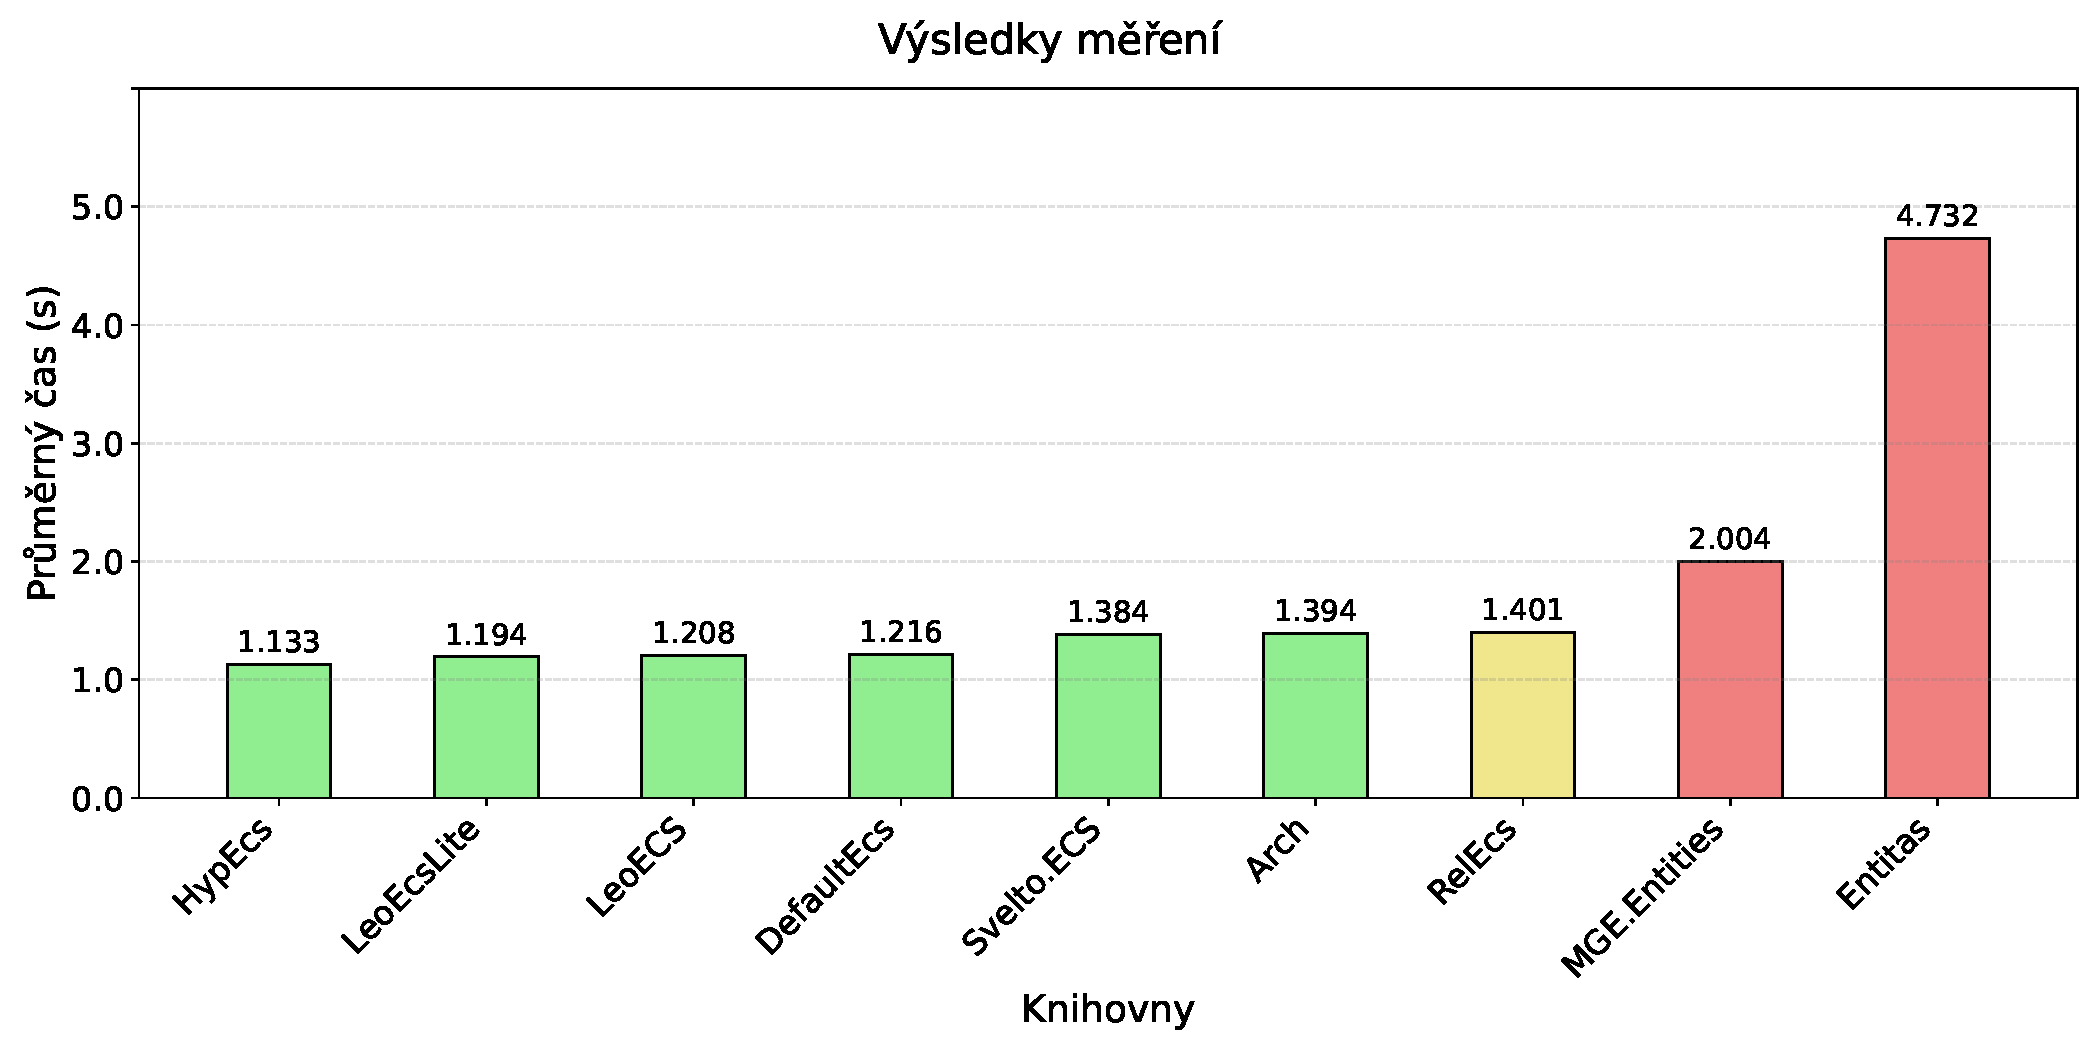
\includegraphics[width=1.0\linewidth]{plots/first_benchmark_results.pdf}
    \caption{Grafy vyobrazující výsledky prvního měření zachycené v tabulce~\ref{tab:first-benchmark-results}. Graf je obarvený podle kategorií ze sekce~\ref{hypothesis}.}
    \label{fig:first-benchmark-results}
\end{figure}

V sekci~\ref{hypothesis} jsme si stanovili hypotézu, podle které mají nejlépe vyjít knihovny z kategorie 1 (viz zelená barva). Poté se mají umístit knihovny z kategorie 2 (viz žlutá barva). A na závěr se mají umístit knihovny z kategorie 3 (viz červená barva). Při nahlédnutí do tabulky~\ref{tab:first-benchmark-results} nebo grafu z obrázku~\ref{fig:first-benchmark-results} je lehké pozorovat, že tomu tak opravdu je. Ovšem je nutné podotknout, že knihovny \textit{Arch} a \textit{RelEcs} mají velmi podobný výsledek a pokud nahlédneme na chybu z tabulky~\ref{tab:first-benchmark-results} tak je možné pozorovat, že časy jsou téměř identické. Vyplývá z toho to, že pro tento počet entit požadavek na to, aby jednotlivé komponenty byli struktury, nemusí nutně vést k velkému výkonnostnímu zlepšení.

\subsection{Druhé měření}
Druhé měření bylo spouštěno s velikostí světa 16384x16384. Výsledky tohoto měření je možné vidět v tabulce~\ref{tab:second-benchmark-results} a grafu znázorněném na obrázku~\ref{fig:second-benchmark-results}.

\begin{table}[!htb]
    \centering\footnotesize\sf
    \begin{tabular}{c c c c}
        \toprule
        knihovna & Průměrný čas & Chyba & StdDev \\
        \midrule
        HypEcs & 7.789 s & 0.1542 s & 0.3044 s \\
        DefaultEcs & 7.958 s & 0.1585 s & 0.3129 s \\
        LeoECS & 8.234 s & 0.1647 s & 0.3011 s \\
        LeoEcsLite & 8.471 s & 0.1670 s & 0.3177 s \\
        Svelto.ECS & 8.589 s & 0.1711 s & 0.3571 s \\
        Arch & 8.938 s & 0.1775 s & 0.4253 s \\
        RelEcs & 13.862 s & 0.2707 s & 0.3424 s \\
        MonoGameExtended.Entities & 20.442 s & 0.2375 s & 0.2222 s \\
        Entitas & 25.908 s & 0.5035 s & 0.6183 s \\
        \bottomrule
    \end{tabular}
    \caption{Výsledky druhého měření pro jednotlivé ECS knihovny.}
    \label{tab:second-benchmark-results}
\end{table}

\begin{figure}[!htb]
    \centering
    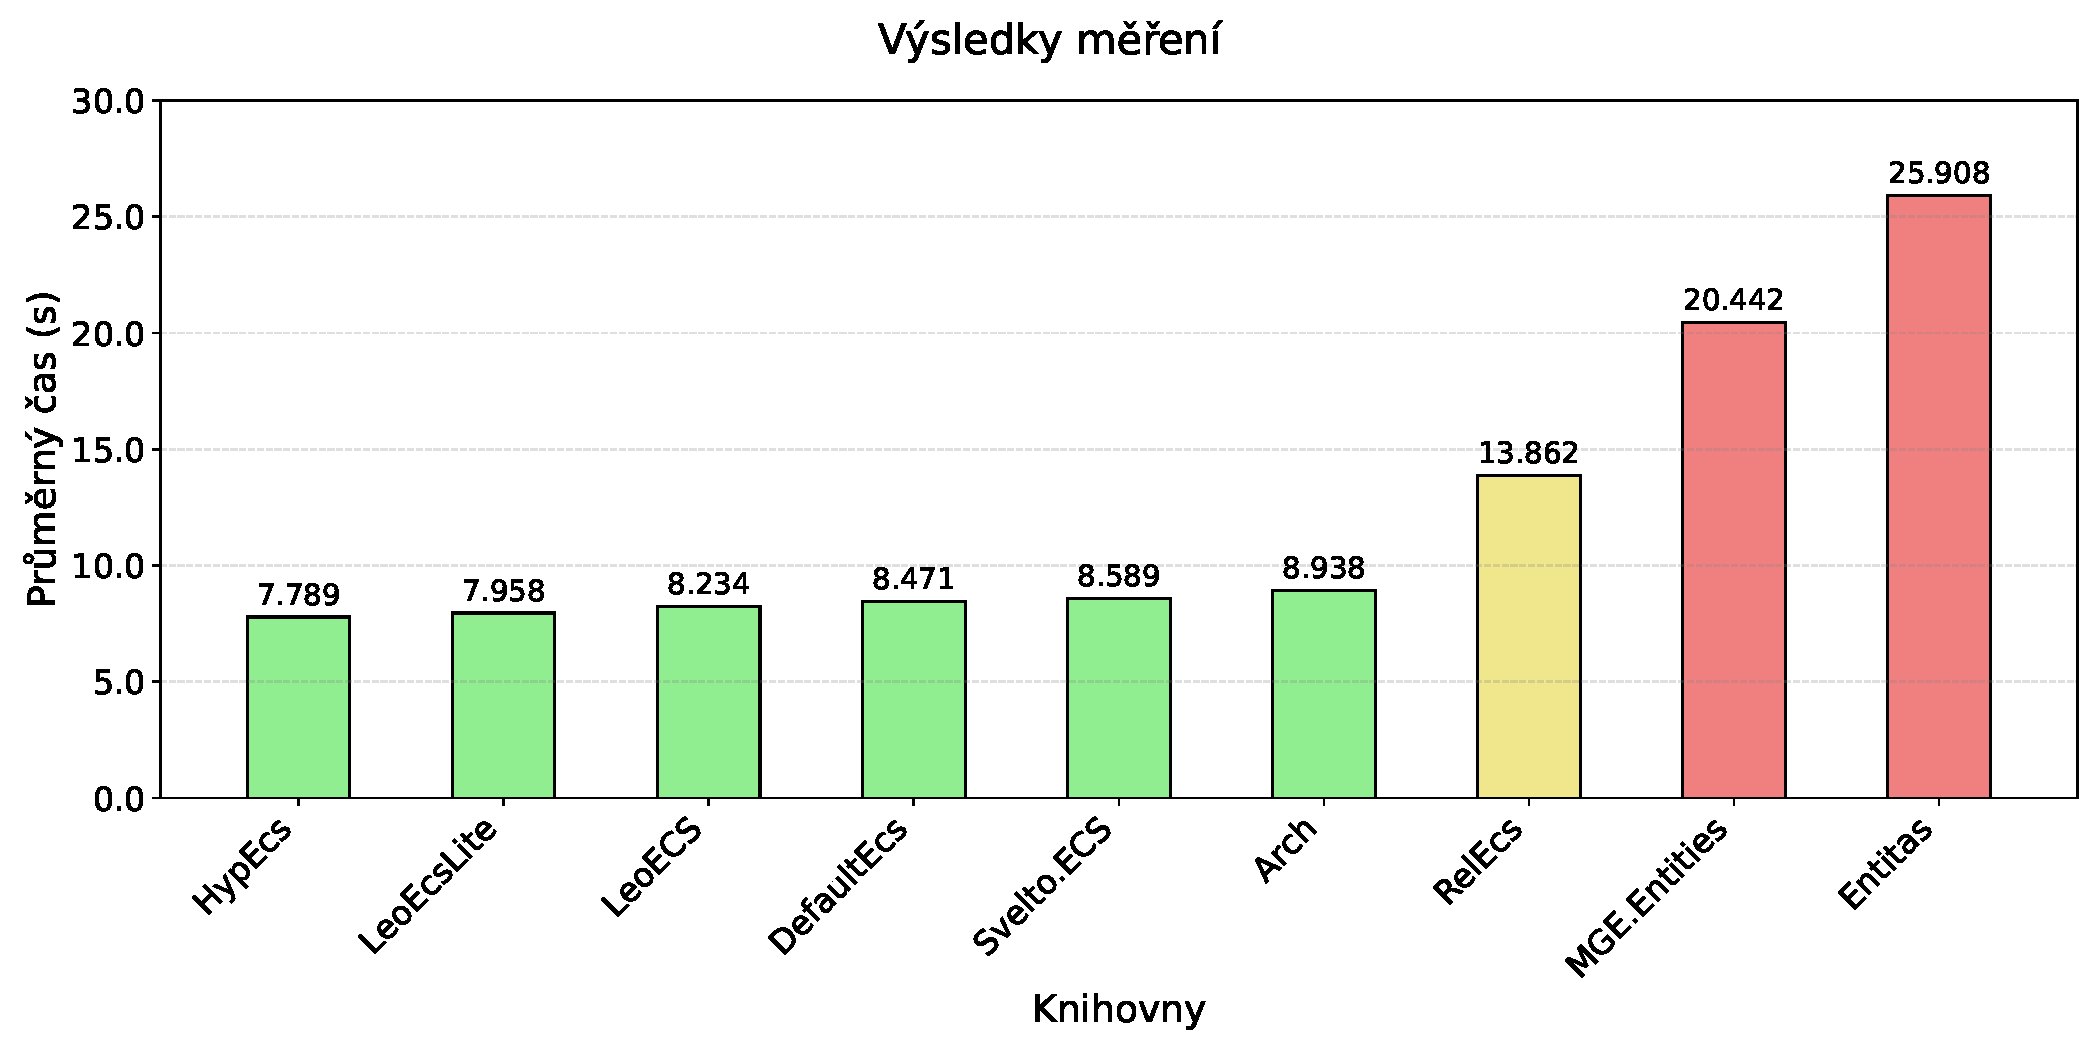
\includegraphics[width=1.0\linewidth]{plots/second_benchmark_results.pdf}
    \caption{Grafy vyobrazující výsledky druhého měření zachycené v tabulce~\ref{tab:second-benchmark-results}. Graf je obarvený podle kategorií ze sekce~\ref{hypothesis}.}
    \label{fig:second-benchmark-results}
\end{figure}

Z tabulky~\ref{tab:second-benchmark-results} i grafu~\ref{fig:second-benchmark-results} je možné vypozorovat významnější rozdíl mezi knihovnami první kategorie (zelená barva) a knihovnou druhé kategorie (žlutá barva). Předpokládáme, že tento rozdíl je způsobený větším počtem \textit{cache misses}, který se pro větší počet entit více projevuje a je způsoben tím, že knihovna \textit{RelEcs} používá třídy namísto struktur pro reprezentaci komponent (viz sekce~\ref{hypothesis}). Lze pozorovat, že hypotéza zde byla také splněna.

\subsection{Třetí měření}
Třetí měření bylo spouštěno s velikostí světa 32768x32768. Výsledky tohoto měření je možné vidět v tabulce~\ref{tab:third-benchmark-results} a grafu znázorněném na obrázku~\ref{fig:third-benchmark-results}.

\begin{table}[!htb]
    \centering\footnotesize\sf
    \begin{tabular}{c c c c}
        \toprule
        knihovna & Průměrný čas & Chyba & StdDev \\
        \midrule
        DefaultEcs & 196.2 s & 3.91 s & 6.63 s \\
        LeoECS & 208.6 s & 3.32 s & 3.10 s \\
        HypEcs & 210.3 s & 2.05 s & 1.82 s \\
        LeoEcsLite & 218.6 s & 3.08 s & 2.88 s \\
        Arch & 220.0 s & 4.27 s & 3.99 s \\
        Svelto.ECS & 229.5 s & 4.52 s & 5.38 s \\
        RelEcs & 236.7 s & 3.60  s & 3.37 s \\
        Entitas & 308.6 s &6.11 s & 6.01 s \\
        MonoGameExtended.Entities & 360.9 s & 1.86 s & 1.74 s \\
        \bottomrule
    \end{tabular}
    \caption{Výsledky třetího měření pro jednotlivé ECS knihovny.}
    \label{tab:third-benchmark-results}
\end{table}

\begin{figure}[!htb]
    \centering
    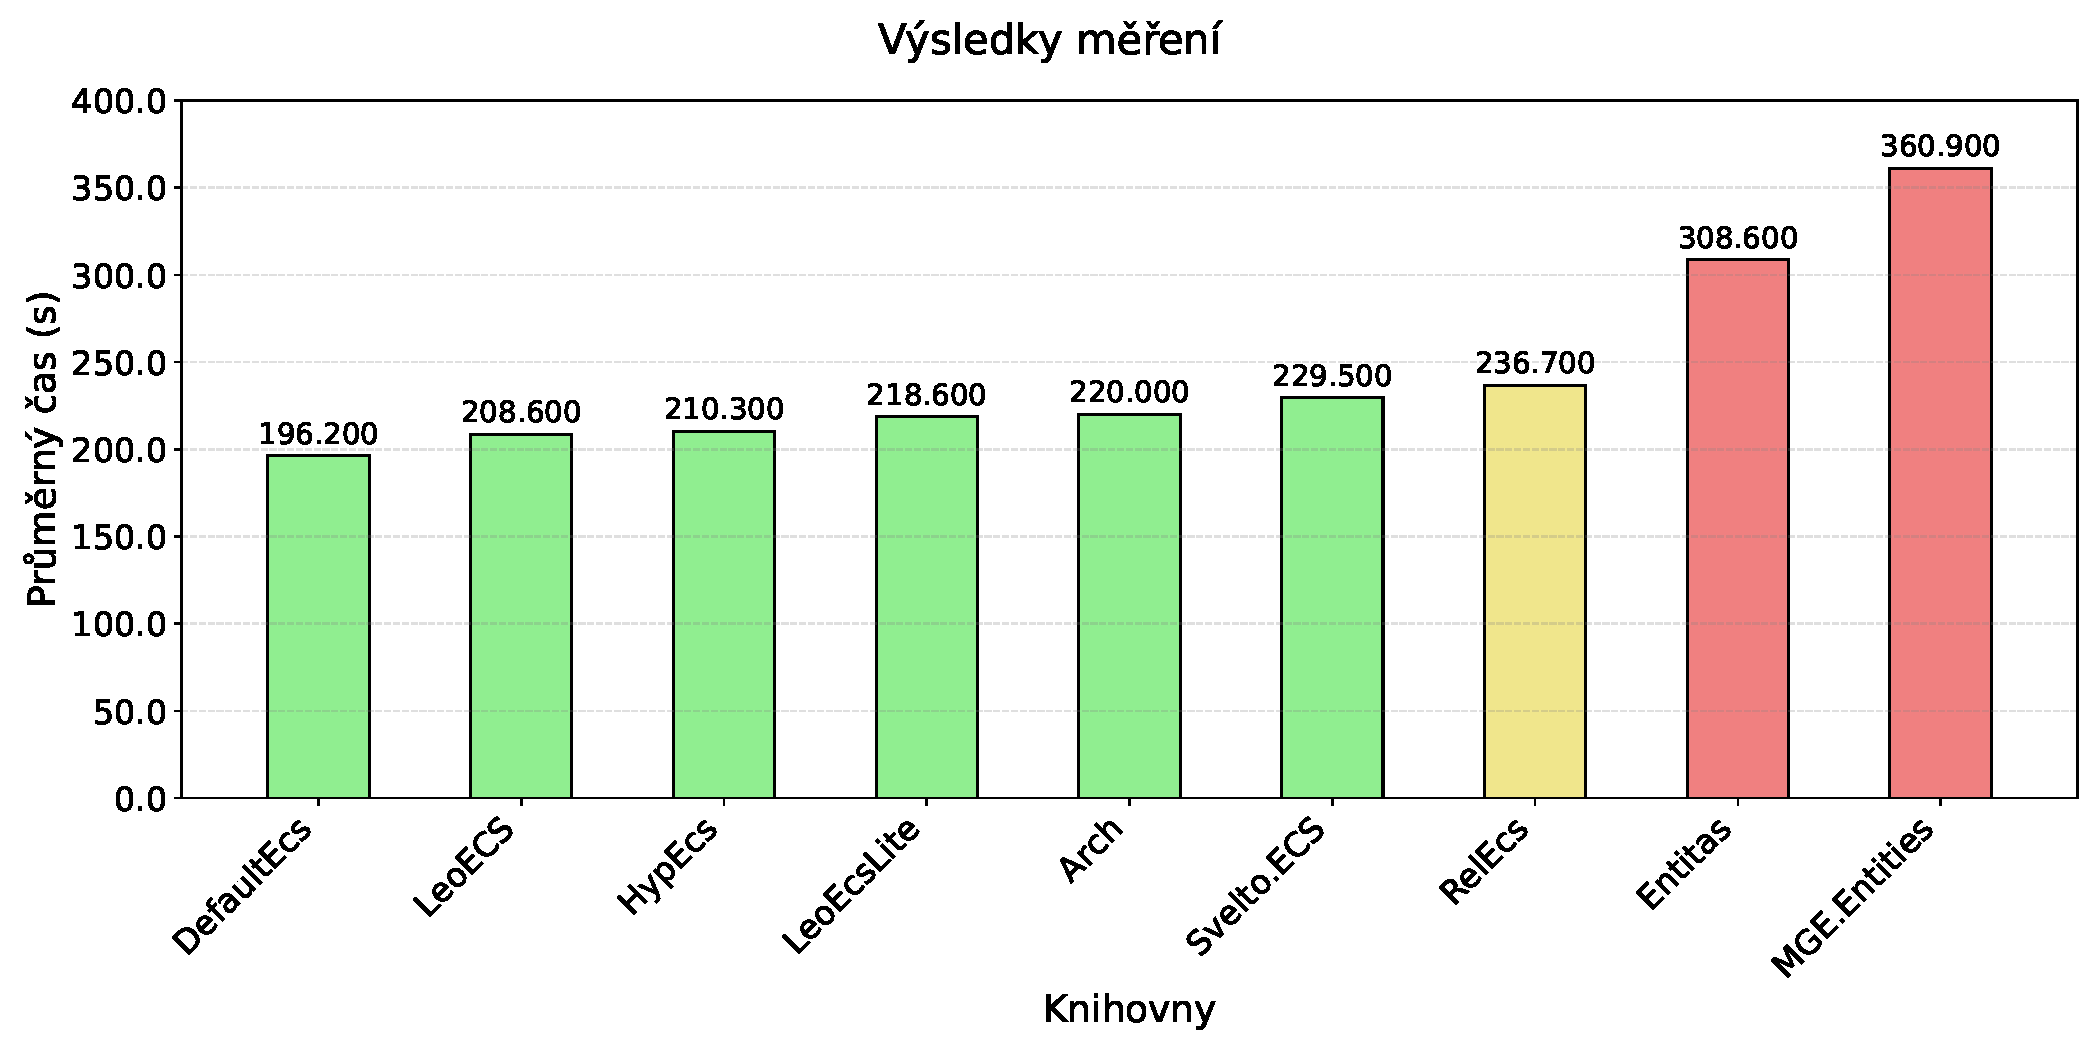
\includegraphics[width=1.0\linewidth]{plots/third_benchmark_results.pdf}
    \caption{Grafy vyobrazující výsledky třetího měření zachycené v tabulce~\ref{tab:third-benchmark-results}. Graf je obarvený podle kategorií ze sekce~\ref{hypothesis}.}
    \label{fig:third-benchmark-results}
\end{figure}

Z tabulky~\ref{tab:third-benchmark-results} i grafu~\ref{fig:third-benchmark-results} lze pozorovat, že výsledky jednotlivých kategorií jsou opět, podobně jako v případě prvního měření, blíže u sebe. Předpokládáme, že hra pro tuto velikost světa tráví spoustu času ve složitějších datových strukturách jako jsou \textit{behavior stromy} a \textit{kd-stromy}, tím pádem knihovny první kategorie (zelená barva) nezískávají tolik výkonu na dobrém využití \textit{cache}. Je možné pozorovat, že hypotéza je stále splněna.

\subsection{Velikosti světa}
Nyní si rozebereme co použité velikosti světů vlastně znamenají. Pro lepší pochopení kontextu autor práce provedl test na realtime strategické hře \textit{Age of Mythology}. Byla spuštěn scénář s prázdnou mapou (bez překážek). Pro frakci byl zvolen bůh Zeus a velikost mapy byla zvolena normální. Vesničan (jednotka villager) z jednoho okraje mapy ke druhému došel za zhruba 60 sekund.

V naší hře se vesničané pohybují rychlostí 120 jednotek za sekundu. Velikost mapy pro první měření je 8192x8192. Vesničan by tedy tento svět zleva doprava přešel za zhruba 68 sekund. Lze tedy tuto velikost světa do jisté míry srovnat s normální velikostí světa ve hře \textit{Age of Mythology}. Velikost mapy pro druhé měření je 16384x16384 a vesničan by tento svět přešel zleva doprava za zhruba 137 sekund. Lze tedy do jisté miry tuto velikost světa považovat za nadstandardní. Velikost mapy pro třetí měření je 32768x32768 a vesničan by tento svět přešel zleva doprava za zhruba 273 sekund. Lze tedy tuto velikost světa do jisté miry považovat za velmi velkou.

\subsection{Závěr měření}
Ve výsledcích pro všechny tři měření je možné pozorovat, že rozdíl mezi ECS knihovnami první kategorie (zelená barva) a ECS knihovnami třetí kategorie (červená barva) není tak velký. Z toho důvodu při výběru ECS knihovny stojí za zvážení ECS knihovny ze třetí kategorie (červená barva).

\subsection{Zajímavé knihovny}
Zajímavou knihovnou je knihovna \textit{Svelto.ECS}, která vyžaduje, aby bylo během kompilace známo, z kterých komponent se jednotlivé entity budou skládat. Je lehké pozorovat že tato omezení nevedla k většímu výkonnostnímu zlepšení oproti ostatním knihovnám z této kategorie.

Knihovny \textit{HypEcs} a \textit{RelEcs} jsou od stejného autora. Autor těchto knihoven udělal nejprve \textit{RelEcs} a poté \textit{HypEcs}. \textit{HypEcs} se mu podařilo udělat rychlejší zejména, protože použil struktury místo třídy pro reprezentaci komponent.

Knihovny \textit{LeoECS} a \textit{LeoEcsLite} jsou od stejného autora. Obě tyto knihovny mají podobný výkon, ovšem při nahlédnutí do výsledků měření projektu \textit{Ecs.Csharp.benchmark}~\cite{EcsCsharpBenchmark} (konkrétně commitu \textit{db67d1d}~\cite{EcsCsharpBenchmarkCommit}), je možné pozorovat, že tyto dvě knihovny se umístili velmi špatně. Hlavním důvodem je to, že autor projektu \textit{Ecs.Csharp.benchmark} použil Nugget balíčky pro tyto knihovny, které byli vytvořeny jiným autorem. Autor projektu \textit{Ecs.Csharp.benchmark} dokonce tvrdí, že tyto balíčky byli sestaveny v debug konfiguraci.

ECS knihovna \textit{Entitas} je na platformě GitHub~\cite{GitHub} nejpopulárnější (má nejvíce hvězdiček) ECS knihovnou pro C\#. I přesto, že v našem měření vyšla nejhůře, její výkon je pořád dost dobrý. K její popularitě také přispívá větší podpora pro herní engine \textit{Unity}~\cite{Unity}.